\documentclass{beamer}
\usepackage{listings} % source code
\usepackage{color}
\usepackage{graphicx}
\usepackage{verbatim}
\usepackage{hyperref}

\usetheme{Dresden}

\title{Necko overview}
\author{Patrick Wang}

\begin{document}

\begin{frame}
  \titlepage
\end{frame}

\begin{frame}{Introduction}
  \begin{itemize}
  \item \textbf{Necko's primary responsibility} is moving data from one location,
    to another location. 
  \item Used to be a standalone module, until Gecko 9.0
  \end{itemize}
\end{frame}

\begin{frame}{Basic component: from a user's perspective}
  \begin{itemize}
  \item URI
    \begin{itemize}
    \item \textbf{URI} represents location
    \item \texttt{nsIURI}, \texttt{nsSimpleURI}, \ldots
    \item \texttt{nsINestedURI} standards for `a uri that contains another uri'
    \end{itemize}
  \item URL
    \begin{itemize}
    \item \textbf{A URL} implements URI interface.
    \item URLs provide getting/setting of paths, hosts, ports, filenames.
    \end{itemize}
  \item Channel
    \begin{itemize}
    \item \texttt{nsIChannel} provides a data access interface which allows you to read or write data from or to a URI
    \end{itemize}
  \end{itemize}
\end{frame}

\begin{frame}{Creating URI and Channel}
  \begin{itemize}
  \item Build \texttt{URI} and \texttt{Channel} though \texttt{nsIOService}
  \end{itemize}
  \begin{center}
    \includegraphics[height=0.7\textheight]{ns-io-service.pdf}
  \end{center}
\end{frame}

\begin{frame}[fragile]
  \frametitle{Add a new protocol}
  To add a new protocol, you will need to implement an \texttt{nsIProtocolHandler}.
\begin{verbatim}
  readonly attribute ACString scheme;
  readonly attribute long defaultPort;
  readonly attribute unsigned long protocolFlags;

  nsIURI newURI(in AUTF8String aSpec,
                in string aOriginCharset,
                in nsIURI aBaseURI);
  nsIChannel newChannel(in nsIURI aURI);
  boolean allowPort(in long port, in string scheme);
\end{verbatim}
\end{frame}

\begin{frame}{Add a new protocol}
  \begin{itemize}
  \item Make contract id of the new protocol handler \texttt{NS\_NETWORK\_PROTOCOL\_CONTRACTID\_PREFIX "my-scheme"}
    \begin{itemize}
    \item Note \texttt{\#define NS\_NETWORK\_PROTOCOL\_CONTRACTID\_PREFIX "@mozilla.org/network/protocol;1?name="}
    \end{itemize}
  \end{itemize}
\end{frame}

\begin{frame}[fragile]
  \frametitle{Add a new protocol}
  \begin{center}
    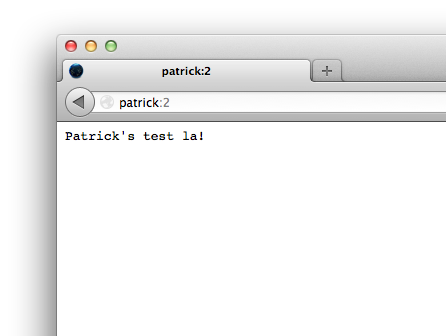
\includegraphics[height=0.7\textheight]{patrick-protocol.png}

    \href{https://github.com/kk1fff/mozilla-central/commit/b5b203307c54862f67774e588475939961258f0a}{Example of adding new protocol}
  \end{center}
\end{frame}

\begin{frame}
  \frametitle{Channel}
  \begin{itemize}
  \item \texttt{nsIChannel} provides a data access interface which allows you to read or write data from or to a URI
  \item Implement \texttt{asyncOpen()} to feed data.
    \begin{itemize}
      \item \texttt{onStartRequest}
      \item \texttt{onDataAvailable}
      \item \texttt{onStopRequest}
    \end{itemize}
  \item \texttt{nsBaseChannel} is very useful base class, \texttt{nsDataChannel} is a good example.
  \end{itemize}
\end{frame}

\begin{frame}[fragile]
  \frametitle{Channel family}
  \begin{center}
    \includegraphics[height=0.8\textheight]{ns-i-channel.pdf}
  \end{center}
\end{frame}

% ---- Inside necko

\begin{frame}{The Socket Transport Service}
  \begin{itemize}
  \item \textbf{MDN:} This interface provides a mapping between a socket type and its associated socket provider instance. One could also use the service manager directly. 
  \item Implements \texttt{nsISocketTransportService}, \texttt{nsIEventTarget}
  \item Can be accessed with \texttt{gSocketTransportService}
  \item As an event target, dispatching event to STS is actually dispatching event to STS thread.
  \end{itemize}
\end{frame}

\begin{frame}[fragile]
  \frametitle{A socket transport}
  \begin{itemize}
  \item \texttt{nsITransport}
    \begin{itemize}
    \item Providing interface of getting input/output stream.
    \end{itemize}
  \item \texttt{nsISocketTransport}
    \begin{itemize}
    \item implements \texttt{nsITransport}
    \item provides methods to open blocking or non-blocking, buffered or unbuffered streams between two end-point in a IP based network.
    \end{itemize}
  \item Getting a \texttt{nsISocketTransport} from \texttt{nsISocketTransportService}
    \begingroup
    \fontsize{8pt}{12pt}\selectfont
\begin{verbatim}
nsISocketTransport createTransport(
    [array, size_is(aTypeCount)]
    in string aSocketTypes,
    in unsigned long aTypeCount,
    // "ssl", "starttls", "udp", or default to tcp
    in AUTF8String aHost,
    in long aPort,
    in nsIProxyInfo aProxyInfo);
\end{verbatim}
\endgroup
  \end{itemize}
\end{frame}

\begin{frame}{Using SocketTransport}
  \begin{itemize}
  \item Call \texttt{SocketTransportService::createTransport}
    \begin{itemize}
    \item Create a \texttt{SocketTransport}
    \item Call \texttt{SocketTransport::Init} to check the socket type list.
    \end{itemize}
  \item Opening I/O stream by calling \texttt{OpenInputStream} and
    \texttt{OpenOutputStream}
    \begin{itemize}
    \item Look up DNS.
    \item Build socket.
    \end{itemize}
  \item Calling asyncWait of \texttt{OpenInput/OutputSocket}
    \begin{itemize}
    \item Registering a callback to being notified when the async stream is ready for I/O.
    \end{itemize}
  \end{itemize}
\end{frame}

\begin{frame}[fragile]
  \frametitle{\texttt{nsSocketTransport} and related classes}
  \begin{center}
    \includegraphics[height=0.8\textheight]{ns-i-socket-transport.pdf}
  \end{center}
\end{frame}

\begin{frame}[fragile]
  \frametitle{Implement your own socket with SocketTransportService}
  \begin{center}
    \includegraphics[height=0.8\textheight]{own-socket.pdf}
  \end{center}
\end{frame}

% ---- Http

\begin{frame}{HTTP}
  \begin{itemize}
  \item \textbf{Protocol Handler $\rightarrow$} \texttt{nsHttpHandler} and \texttt{nsHttpsHandler}.
  \item \textbf{newURI} creates a \texttt{StandardURL} instance with the url.
  \item \textbf{newChannel} creates an \texttt{nsHttpChannel}, then calls its \texttt{Init()} function.
  \end{itemize}
\end{frame}

\begin{frame}{HTTP Channel}
  \texttt{HttpChannel::Init()}  Simply calls \texttt{HttpBaseChannel::Init()}
  \begin{enumerate}
  \item \textbf{Set up ssl config} by scheme (http/https).
  \item \textbf{Initialize header} for request method, host/port pair and standard request headers (user-agent, accept language, accept encoding, accept type, DNT).
  \item \textbf{Initialize proxy config} with \texttt{ProxyInfo}.
  \end{enumerate}
\end{frame}

\begin{frame}{HTTP Channel}
  \texttt{HttpChannel::AsyncOpen}
  \begin{enumerate}
  \item Adding cookies into header.
  \item Setting up listener and context.
  \item Resolve proxy if proxy info is not set to current channel. (call \texttt{ProtocolProxyService})
  \item After proxy resolved, call \texttt{BeginConnect}
  \end{enumerate}
\end{frame}

\begin{frame}{Http Channel}
  \texttt{HttpChannel::BeginConnect()}
  \begin{enumerate}
    \item Building \texttt{nsHttpConnectionInfo}, which includes proxy info, host, port, ssl.
    \item Building \texttt{nsAuthProvider}, and add auth into request header.
    \item Calling \texttt{NS\_HTTP\_ON\_MODIFY\_REQUEST\_TOPIC} and subject is the channel. It's a chance to modify the channel.
    \item Setting connection header \texttt{keep-alive}/\texttt{close}.
    \item Calling \texttt{Connect()}, finally.
  \end{enumerate}
\end{frame}

\begin{frame}{Http Channel}
  \texttt{HttpChannel::Connect()}
  \begin{enumerate}
  \item Try to use \texttt{SpeculativeConnect}
  \item Checking if we need to load cache.
  \item Calling \texttt{ContinueConnect()}
  \end{enumerate}
\end{frame}

\begin{frame}{Http Channel}
  \texttt{HttpChannel::ContinueConnect()}
  \begin{enumerate}
  \item Format \texttt{requestURI}(path without hash), set it to header.
  \item Create \texttt{nsHttpTransaction}
  \item Call \texttt{SetupTransaction}
    \begin{enumerate}
    \item \texttt{nsHttpTransaction::Init()}
      \begin{enumerate}
      \item From request header + request content stream.
      \end{enumerate}
    \item Create a \texttt{nsImputStreamPump} to fetch response data.
    \end{enumerate}
  \item Call \texttt{nsHttpHandler::InitiateTransaction()}
    \begin{enumerate}
    \item Adding transaction into \texttt{nsHttpConnectionMgr::AddTransaction}
    \item Doing actual IO.
    \end{enumerate}
  \end{enumerate}
\end{frame}

\begin{frame}{AddTransaction}
  \begin{enumerate}
  \item Post OnMessageNewTransaction to STS thread (async).
  \item Try to get a existing \texttt{nsHttpConnection} for the \texttt{HttpTransaction}, or create one if there is not an \texttt{nsHttpConnection} available for the transaction.
  \item \texttt{nsHttpConnection} creates transport and handles ssl.
  \end{enumerate}
\end{frame}

\begin{frame}{so...}
  \large Questions?
\end{frame}

\end{document}

